\let\negmedspace\undefined
\let\negthickspace\undefined
\documentclass[journal,12pt,twocolumn]{IEEEtran}
%\documentclass[conference]{IEEEtran}
%\IEEEoverridecommandlockouts
% The preceding line is only needed to identify funding in the first footnote. If that is unneeded, please comment it out.
\usepackage{svg}
\usepackage{tikz, pgfplots}
\usepackage{cite}
\usepackage{amsmath,amssymb,amsfonts,amsthm}
\usepackage{algorithmic}
\usepackage{graphicx,wrapfig}
\usepackage{textcomp}
\usepackage{xcolor}
\usepackage{txfonts}
\usepackage{listings}
\usepackage{enumitem}
\usepackage{mathtools}
\usepackage{gensymb}
\usepackage[breaklinks=true]{hyperref}
\usepackage{tkz-euclide} % loads  TikZ and tkz-base
\usepackage{listings}


\usetikzlibrary{positioning}
%
%\usepackage{setspace}
%\usepackage{gensymb}
%\doublespacing
%\singlespacing

%\usepackage{graphicx}
%\usepackage{amssymb}
%\usepackage{relsize}
%\usepackage[cmex10]{amsmath}
%\usepackage{amsthm}
%\interdisplaylinepenalty=2500
%\savesymbol{iint}
%\usepackage{txfonts}
%\restoresymbol{TXF}{iint}
%\usepackage{wasysym}
%\usepackage{amsthm}
%\usepackage{iithtlc}
%\usepackage{mathrsfs}
%\usepackage{txfonts}
%\usepackage{stfloats}
%\usepackage{bm}
%\usepackage{cite}
%\usepackage{cases}
%\usepackage{subfig}
%\usepackage{xtab}
%\usepackage{longtable} 
%\usepackage{multirow}
%\usepackage{algorithm}
%\usepackage{algpseudocode}
%\usepackage{enumitem}
%\usepackage{mathtools}
%\usepackage{tikz}
%\usepackage{circuitikz}
%\usepackage{verbatim}
%\usepackage{tfrupee}
%\usepackage{stmaryrd}
%\usetkzobj{all}
%    \usepackage{color}                                            %%
%    \usepackage{array}                                            %%
%    \usepackage{longtable}                                        %%
%    \usepackage{calc}                                             %%
%    \usepackage{multirow}                                         %%
%    \usepackage{hhline}                                           %%
%    \usepackage{ifthen}                                           %%
  %optionally (for landscape tables embedded in another document): %%
%    \usepackage{lscape}     
%\usepackage{multicol}
%\usepackage{chngcntr}
%\usepackage{enumerate}

%\usepackage{wasysym}
%\newcounter{MYtempeqncnt}
\DeclareMathOperator*{\Res}{Res}
%\renewcommand{\baselinestretch}{2}
\renewcommand\thesection{\arabic{section}}
\renewcommand\thesubsection{\thesection.\arabic{subsection}}
\renewcommand\thesubsubsection{\thesubsection.\arabic{subsubsection}}

\renewcommand\thesectiondis{\arabic{section}}
\renewcommand\thesubsectiondis{\thesectiondis.\arabic{subsection}}
\renewcommand\thesubsubsectiondis{\thesubsectiondis.\arabic{subsubsection}}

% correct bad hyphenation here
\hyphenation{op-tical net-works semi-conduc-tor}
\def\inputGnumericTable{}                                 %%

\lstset{
%language=C,
frame=single, 
breaklines=true,
columns=fullflexible
}
%\lstset{
%language=tex,
%frame=single, 
%breaklines=true
%}

\begin{document}
%


\newtheorem{theorem}{Theorem}[section]
\newtheorem{problem}{Problem}
\newtheorem{proposition}{Proposition}[section]
\newtheorem{lemma}{Lemma}[section]
\newtheorem{corollary}[theorem]{Corollary}
\newtheorem{example}{Example}[section]
\newtheorem{definition}[problem]{Definition}
%\newtheorem{thm}{Theorem}[section] 
%\newtheorem{defn}[thm]{Definition}
%\newtheorem{algorithm}{Algorithm}[section]
%\newtheorem{cor}{Corollary}
\newcommand{\BEQA}{\begin{eqnarray}}
\newcommand{\EEQA}{\end{eqnarray}}
\newcommand{\define}{\stackrel{\triangle}{=}}
\newcommand\tab[1][1cm]{\hspace*{#1}}
\bibliographystyle{IEEEtran}
%\bibliographystyle{ieeetr}


\providecommand{\mbf}{\mathbf}
\providecommand{\pr}[1]{\ensuremath{\Pr\left(#1\right)}}
% Added from https://raw.githubusercontent.com/gadepall/digital-communication/main/probability/trans.tex %%
\newcommand*{\permcomb}[4][0mu]{{{}^{#3}\mkern#1#2_{#4}}}
\newcommand*{\perm}[1][-3mu]{\permcomb[#1]{P}}
\newcommand*{\comb}[1][-1mu]{\permcomb[#1]{C}}
\providecommand{\gauss}[2]{\mathcal{N}
\ensuremath{\left(#1,#2\right)}}
%%
\providecommand{\qfunc}[1]{\ensuremath{Q\left(#1\right)}}
\providecommand{\sbrak}[1]{\ensuremath{{}\left[#1\right]}}
\providecommand{\lsbrak}[1]{\ensuremath{{}\left[#1\right.}}
\providecommand{\rsbrak}[1]{\ensuremath{{}\left.#1\right]}}
\providecommand{\brak}[1]{\ensuremath{\left(#1\right)}}
\providecommand{\lbrak}[1]{\ensuremath{\left(#1\right.}}
\providecommand{\rbrak}[1]{\ensuremath{\left.#1\right)}}
\providecommand{\cbrak}[1]{\ensuremath{\left\{#1\right\}}}
\providecommand{\lcbrak}[1]{\ensuremath{\left\{#1\right.}}
\providecommand{\rcbrak}[1]{\ensuremath{\left.#1\right\}}}
\theoremstyle{remark}
\newtheorem{rem}{Remark}
\newcommand{\sgn}{\mathop{\mathrm{sgn}}}
\providecommand{\abs}[1]{\(left\)vert#1\(right\)vert}
\providecommand{\res}[1]{\Res\displaylimits_{#1}}
\providecommand{\norm}[1]{\(left\)lVert#1\(right\)rVert}
%\providecommand{\norm}[1]{\lVert#1\rVert}
\providecommand{\mtx}[1]{\mathbf{#1}}
\providecommand{\mean}[1]{E\(left\)[ #1 \(right\)]}
\providecommand{\fourier}{\overset{\mathcal{F}}{ \rightleftharpoons}}
%\providecommand{\hilbert}{\overset{\mathcal{H}}{ \rightleftharpoons}}
\providecommand{\system}{\overset{\mathcal{H}}{ \longleftrightarrow}}
%\newcommand{\solution}[2]{\textbf{Solution:}{#1}}
\newcommand{\solution}{\noindent \textbf{Solution: }}
\newcommand{\cosec}{\,\text{cosec}\,}
\providecommand{\dec}[2]{\ensuremath{\overset{#1}{\underset{#2}{\gtrless}}}}
\newcommand{\myvec}[1]{\ensuremath{\begin{pmatrix}#1\end{pmatrix}}}
\newcommand{\mydet}[1]{\ensuremath{\begin{vmatrix}#1\end{vmatrix}}}

\let\vec\mathbf

\vspace{3cm}

\title{
\textbf {Assignment 2}\\ \large \textbf{AI1110}: Probability and Random Variables\\Indian Institute of Techonology, Hyderabad
}
\author{Gunethra Bommineni$^{*}$% <-this % stops a space
	\thanks{*The student is with the Department
		of Electrical Engineering, Indian Institute of Technology, Hyderabad
		502285 India e-mail: ee22btech11205@iith.ac.in.}
  }

\maketitle

\newpage


\bigskip
\renewcommand{\thefigure}{\theenumi}
\renewcommand{\thetable}{\theenumi}
\textbf{10.15.1.12}
A game of chance consists of spinning an arrow
which comes to rest pointing at one of the numbers
1, 2, 3, 4, 5, 6, 7, 8 (see Fig. 4), and these are equally
likely outcomes. What is the probability that it will
point at:
\begin{enumerate}[label=(\roman*)]
\item 
8?
\item 
an odd number?
\item 
a number greater than 2?
\item 
a number less than 9?
\end{enumerate}

\begin{figure} [p h]
    \setcounter{figure}{0}
    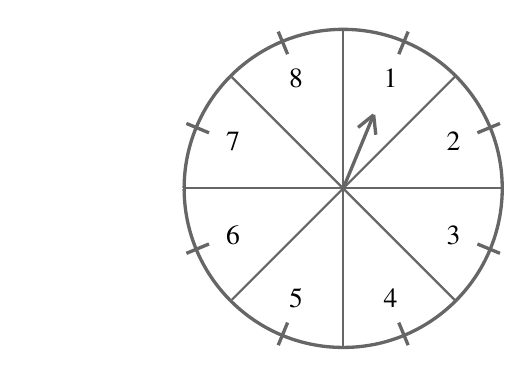
\begin{tikzpicture}
    
	%outline%
	\filldraw[color=black!60, fill=white, very thick](2,0) circle (2.02);
	\draw[black!60, thick] (2,-2) -- (2,2);
	\draw[white!60, thin] (4,0) -- (-2,0);
	\draw[black!60, thick] (4,0) -- (-0.04,0);
	\draw[black!60, thick] (0.58578643762,-1.41421356237) -- (3.41421356237,1.41421356237);
	\draw[black!60, thick] (3.41421356237,-1.41421356237) -- (0.58578643762,1.41421356237);
	%%
	
	%Numbers%
	\node at (2.6,1.4) [] {1};
	\node at (3.4,0.6) [] {2};
	\node at (3.4,-0.6) [] {3};
	\node at (2.6,-1.4) [] {4};
	\node at (1.4,-1.4) [] {5};
	\node at (0.6,-0.6) [] {6};
	\node at (0.6,0.6) [] {7};
	\node at (1.4,1.4) [] {8};
	%%
	
	%Pointer%
	\draw[black!60, very thick] (2,0) -- (2.3867594105005, 0.9337198142057);
	\draw[black!60, very thick] (2.3867594105005, 0.9337198142057) -- (2.4141344385572, 0.6810718956735);
	\draw[black!60, very thick] (2.3867594105005, 0.9337198142057) -- (2.1887532860797, 0.774427825733);
	%%

	%outcome%
	\draw[black!60, very thick] (2.7059955543533, 1.7044240422949) -- (2.824738175107, 1.9910940877502); %1 
	\draw[black!60, very thick] (3.9910940877502, 0.824738175107) -- (3.7044240422949, 0.7059955543533); %2
	\draw[black!60, very thick] (3.9910940877502, -0.824738175107) -- (3.7044240422949, -0.7059955543533); %3
	\draw[black!60, very thick] (2.7059955543533, -1.7044240422949) -- (2.824738175107, -1.9910940877502); %4
	\draw[black!60, very thick] (1.17526182489, -1.9910940877502) -- (1.29400444565, -1.7044240422949); %5
	\draw[black!60, very thick] (0.00890591224, -0.824738175107) -- (0.2955759577, -0.7059955543533); %6
	\draw[black!60, very thick] (0.2955759577, 0.7059955543533) -- (0.00890591224, 0.824738175107); %7
	\draw[black!60, very thick] (1.29400444565, 1.7044240422949) -- (1.17526182489, 1.9910940877502); %8
	%%


    \end{tikzpicture}
\caption{Spinner}
\end{figure}


\textbf{Solution:}
Let X be a random variable defined as the value given by the pointer. The distribution is unform since all the outcomes are equally likely.
\begin{align}
    \therefore \pr{X=i}=\frac{1}{8}
\end{align}
Let $F_{X}\brak{i}$ be the Cumulative distribution function(CDF) such that;
\begin{align}
    F_{X} \brak{i} &= P(X \leq i)\\
    &=
    \begin{cases}
        0, & i \le 0\\
        \frac{i}{8} & 1 \le i \le 8\\
        1, & i \ge 9
    \end{cases}
\end{align}

\begin{figure}
    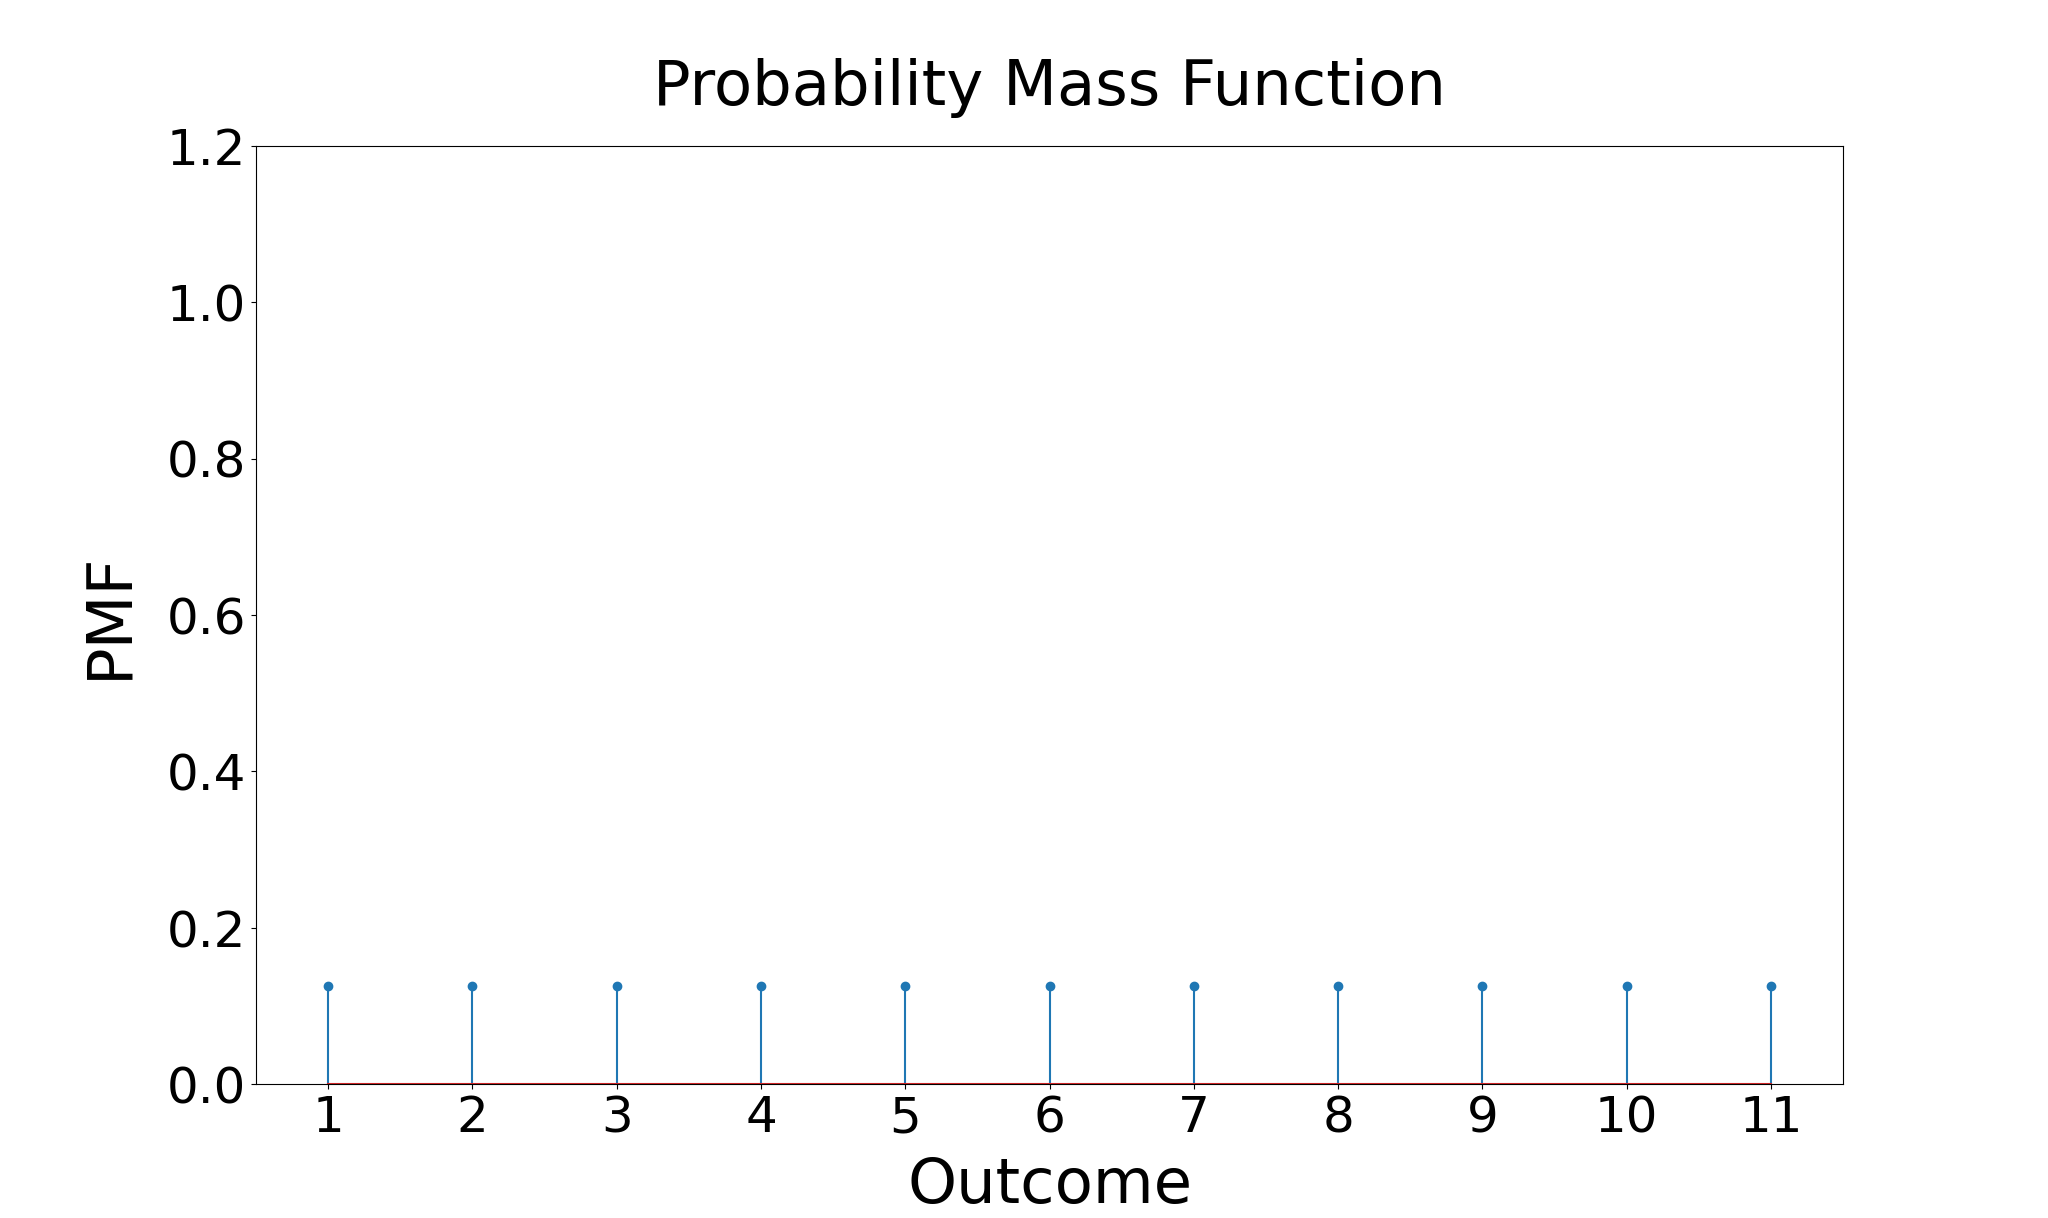
\includegraphics[scale=0.15]{code/pmf.png}
\caption{Plot of Probability Mass Function}
\end{figure}

\begin{figure}
    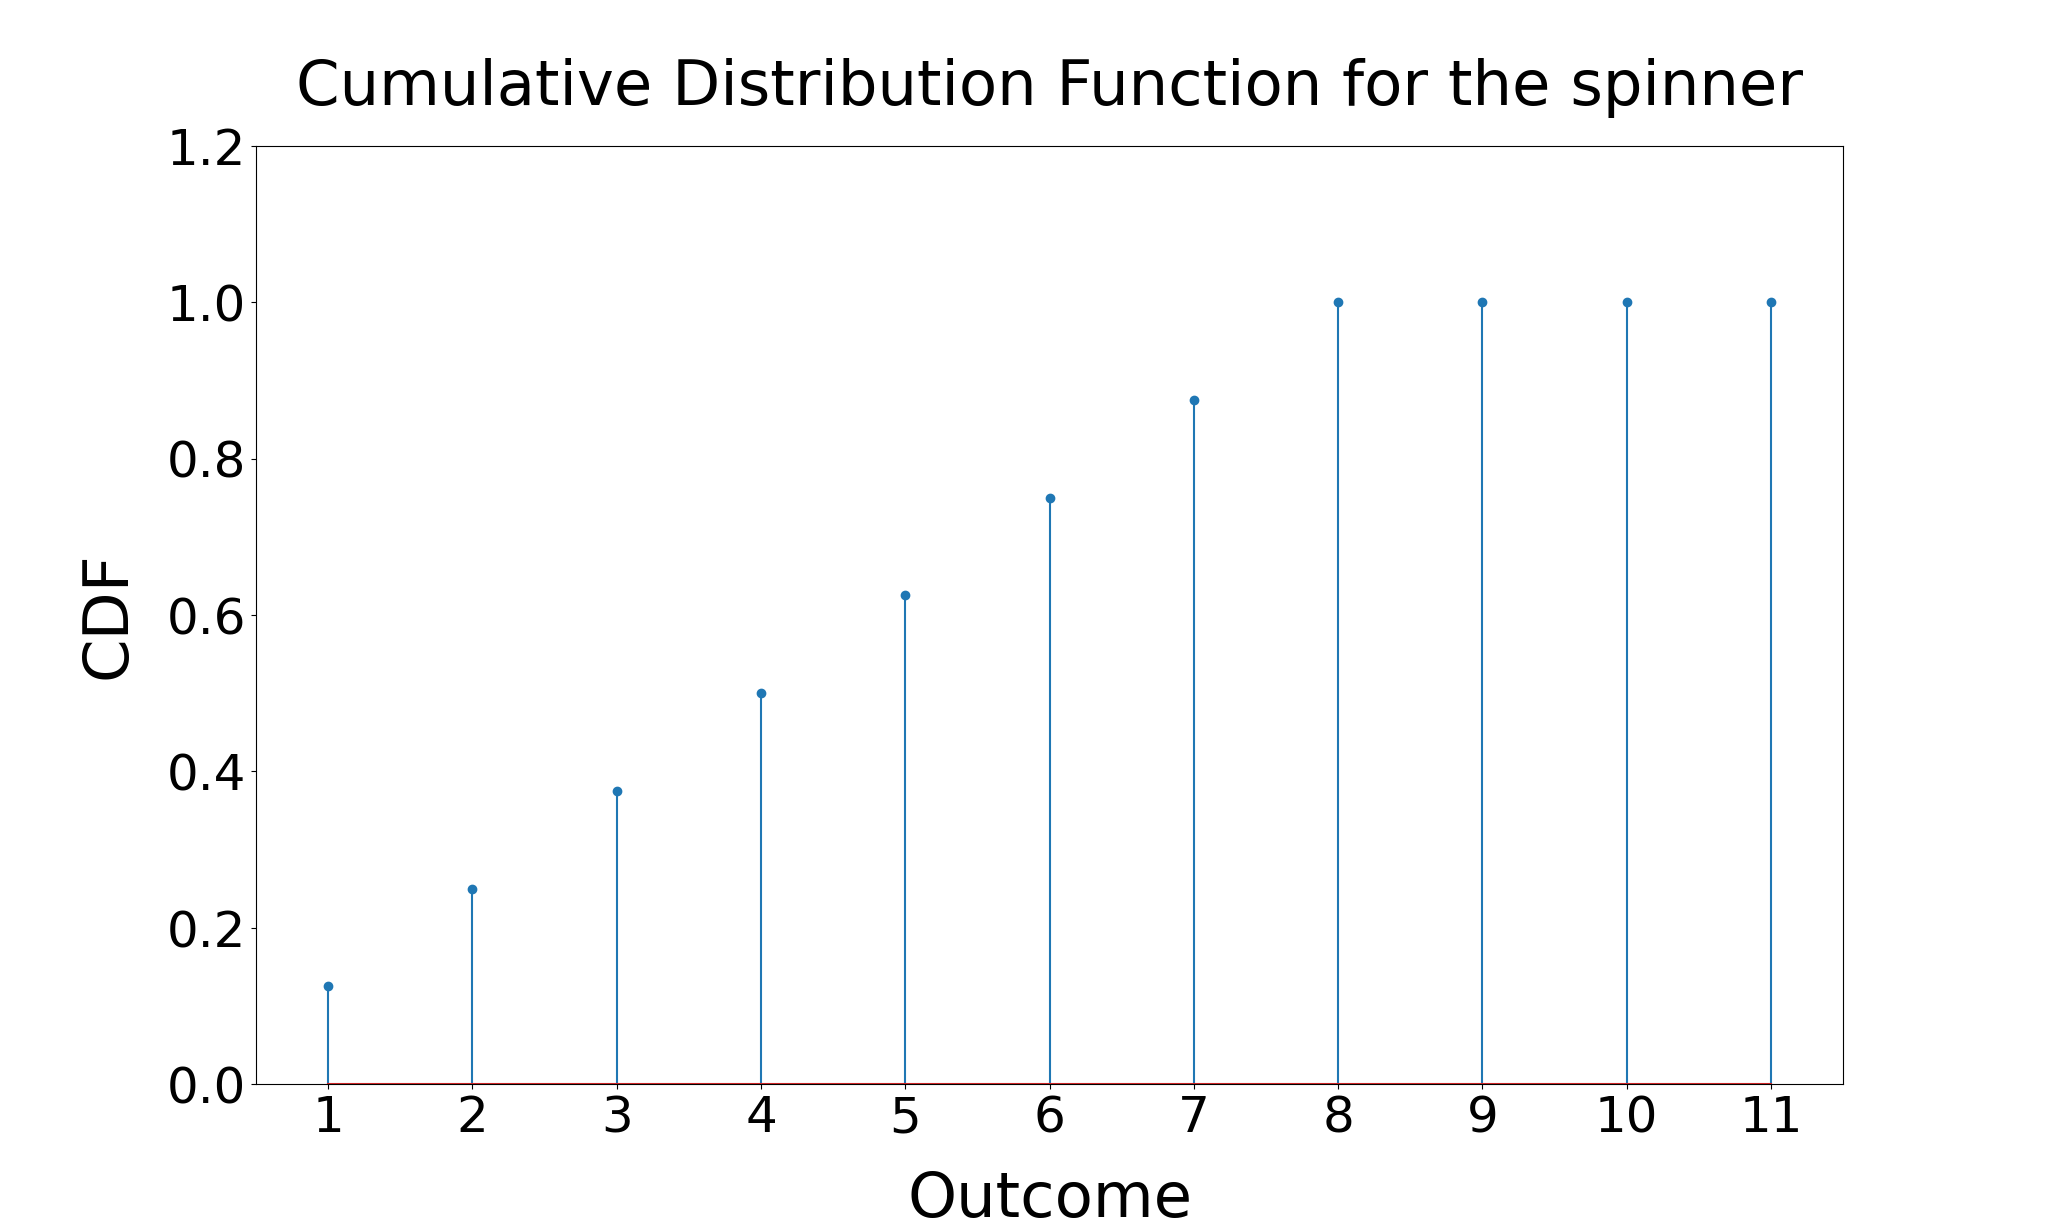
\includegraphics[scale=0.15]{code/cdf.png}
\caption{Plot of Cumulative Distribution Function}
\end{figure}

See python code for PMF and CDF plots:\cite{plot}

\begin{enumerate}[label=(\roman*)]
\item 
For i = 8, required probability is equivalent to;
\begin{align}
    \pr{X=8} &= \frac{1}{8}\\
    &= 0.125
\end{align}
\item 
For i being odd, required probability is equivalent to;
\begin{multline}
    \pr{X=\cbrak{1,3,5,7}} &= \frac{4}{8}\\
    &= 0.5
\end{multline}

\item 
For i greater than 2, required probability is equivalent to;
\begin{align}
    \pr{X > 2} &= 1 - \pr{X \le 2}\\
    &= 1 - \brak{F_{X}\brak{2}-F_{X}\brak{0}}\\
    &= \frac{6}{8}= 0.75
\end{align}

\item 
For i less than 9, required probability is equivalent to;
\begin{align}
    \pr{1 \le X < 9} &= F_{X}\brak{8}-F_{X}\brak{0}\\
    &= \frac{8}{8}= 1
\end{align}

\end{enumerate}
See simulation using python:\cite{simulation}
\bibliography{bibliography}
\end{document}
